\documentclass{beamer}

\usetheme{default}
\usecolortheme{default}
\usefonttheme{default}

\title{Low-Level Network Programming and Operating Systems Development}
\author{Jacob Bates}
\institute{Da Vinci Science High School}

\begin{document}

\section{Introduction}

    \begin{frame}
        \titlepage
    \end{frame}

    \begin{frame}{Contents}
        \tableofcontents
    \end{frame}

\section{Project}

    \begin{frame}{Project}
        The goal of this project was to implement a \textbf{network driver} and \textbf{network stack} at the \textbf{base level}.
        This was to be accomplished through writing an \textbf{operating system} for the \textbf{IA-32 Architecture} in the \textbf{C Programming Language}.
        The system was to be implemented as a \textbf{TFTP Storage Server}.\\
        \rule{0.5\textwidth}{0.5pt}\\
        I took on this project because I was already very involved with and interested in low-level programming, and I wanted to learn more specifically about networking.
    \end{frame}

\section{Hardware}

    \begin{frame}{Network Adaptor}
        \textbf{Realtek RTL8139}\\
        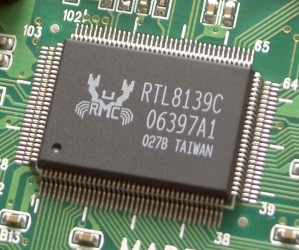
\includegraphics[height=125pt]{Realtek_RTL8139C.jpg}\\
        \rule{0.5\textwidth}{0.5pt}\\
        \begin{itemize}
            \item Widely Used on Older Machines
            \item Easier to Program
            \item Inexpensive
        \end{itemize}
    \end{frame}

    \begin{frame}{Technical Details}

    \end{frame}

\end{document}
